\documentclass[12pt]{article}
\usepackage[T2A]{fontenc}
\usepackage[utf8]{inputenc}
\usepackage[english,russian]{babel}
\usepackage{amssymb,amsmath,amsthm, mathtools}
\usepackage{subfigure}
\newcommand\independent{\protect\mathpalette{\protect\independenT}{\perp}}
\DeclareMathOperator{\trace}{trace}
\def\independenT#1#2{\mathrel{\rlap{$#1#2$}\mkern2mu{#1#2}}}


\newtheorem{note}{Замечание}
\begin{document}


\section{Математическая постановка задачи} 
Марковское случайное поле (MRF) это графическая модель совместного распределения. Иными словами, это неориентированный граф $G = (\mathcal{N}, \mathcal{E})$, где множество вершин $\mathcal{N}$ -- это множество случайных величин. 
Множество случайных величин связанных с множеством вершин $S$ будем обозначать $X_S$. Ребра $\mathcal{E}$ указывают на условную независимость: пусть $A, B$ и $C$ --- непересекающиеся подмножества вершин. Говорят, что $X_A$ условно независимо с $X_B$ при условии $X_C$, если не существует путей из вершины множества $A$ в вершину множества $B$, которая не проходит через $C$ (рисунок \ref{fig:mrf} (a)). Будем обозначать условную независимость как $X_A \independent X_B \mid X_C$.

Будем обозначать всех соседей вершины $n$ за $N_n$: 
\begin{equation*}
N_n = \{ m \in \mathcal{N} \mid (m, n) \in \mathcal{E}\}.
\end{equation*}
Имеет место Марковское свойство (отсюда и название):
\begin{equation*}
P(X_n \mid X_\mathcal{N} - X_n) = P(X_n \mid X_{N_n})
\end{equation*}

На рисунке \ref{fig:example} при условии серых вершин черная условно независима с остальными.

\begin{figure}[hhh]
\centering
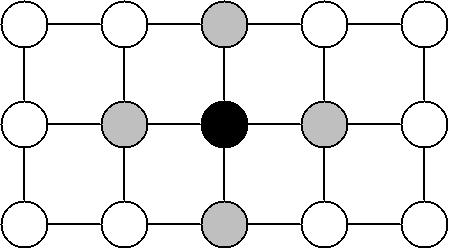
\includegraphics[width=.5\linewidth]{figures/blanket.jpg}
\label{fig:example}
\caption{Пример графа для пиксельного изображения}
\end{figure}


Далее, реализацию Марковского случайного поля будем обозначать $x$ с индексом, соответсвующем подмножеству вершин.
Распределение Гиббса на графе имеет вид:
\begin{equation}
p(x) = \frac{1}{Z} \prod\limits_{C \in \mathcal{C}} \psi_C(x_C), 
\label{eqn:jointdens}
\end{equation}
где $Z  = \sum\limits_{x \in \mathcal{X}} \prod\limits_{C \in \mathcal{C}} \psi_C(x_C)$.
При этом $\psi_C(\cdot)$ -- это положительные функции (не обязательно плотности), а $C$ --- максимальные клики (полные подграфы, которые перестают быть полными при добавлении новой вершины из графа, на рисунке \ref{fig:mrf} (b) обозначены синим цветом).

Чаще всего $\psi_C(x_C) = exp(-V_C(x_C)/T)$ и тогда совместная плотность принимает вид:
\begin{equation}
p(x) = \frac{1}{Z} \exp\left(-\frac{1}{T} U(x)\right),   
\end{equation}
$U(x) = \sum_{C \in \mathcal{C}}V_C(x_C)$ будем называть функцией энергии.
Теорема  Хаммерсли-Клиффорда утверждает, что любое совместное распределение может быть записано как произведение распределене Гиббса. Более того, для любого распределения Гиббса существует МRF для которой оно является его совместным распределением. Таким образом совместное распределение графа можно записывать в виде \eqref{eqn:jointdens}.


\begin{figure}[hhh]
\centering
\subfigure[Условная независимость]{
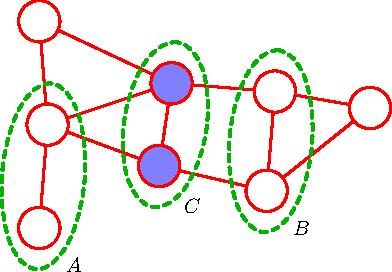
\includegraphics[width=.3\linewidth]{figures/Figure827.pdf}
}
\subfigure[Граф с кликами]{
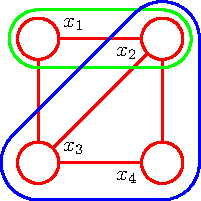
\includegraphics[width=.3\linewidth]{figures/Figure829.pdf}
}\label{fig:mrf}
\caption{Примеры}
\end{figure}

Существует несколько задач, связанных с MRF 
\begin{enumerate}
\item Оценка параметров совместного распределения (в предположении, что известна структура графа)
\item Оценка структуры графа
\item Определение вероятности данной конфигурации графа (выборки)
\item Определение наиболее вероятной конфигурации при условии некоторой информации
\end{enumerate}
Обычно первая задача решается оптимизацией функционала правдоподобия.

Рассмотрим последнюю задачу на примере очисти изображения от шума.

\section{Пример 1}
Рассмотрим граф со структурой, представленной на рисунке \ref{fig:example}.
Пусть каждая вершина $Y_i$ представляет собой пиксель от 0 до 255.
Рассмотрим зашумленное изображение 
\begin{gather*}
Y_i = X_i + e_i, 
\end{gather*}
где $e_i \sim \mathcal{N}(0, \sigma^2)$.
Тогда стоит задача найти 
\begin{gather*}
arg\max\limits_X P(X \mid Y).
\end{gather*}

По формуле условной вероятности (тут $X = X_\mathcal{N}$)
\begin{gather*}
P(X\mid Y) = \frac{P(Y\mid X)P(X)}{P(Y)}.
\end{gather*}
Учитывая, что $P(Y_i\mid X_i) =  P(Y_i\mid X)$ и что $Y_i$ независимы, при условии, что все элементы $X$ фиксированы, получаем
\begin{gather*}
P(X\mid Y) = \frac{\prod P(Y_i\mid X_i)P(X)}{P(Y)}.
\end{gather*}

При этом 
\begin{gather*}
P(Y_i\mid X_i) = \frac{1}{\sqrt{2\pi\sigma^2}} \exp(\frac{(Y_i - X_i)}{2\sigma^2}).
\end{gather*}
Таким образом, 
\begin{gather*}
V_C(X_i) = \frac{(Y_i - X_i)^2}{2\sigma^2}.
\end{gather*}

\end{document}